\documentclass{article}
\usepackage{amsmath}
\usepackage{amsfonts}
\usepackage{geometry}
\usepackage{graphicx}
\usepackage{float}
\geometry{margin=1in}
\title{Mathematical Formulation and code explanation of Variational Autoencoders}

\begin{document}
\maketitle

\section*{Architecture}

\begin{figure}[H]
    \centering
    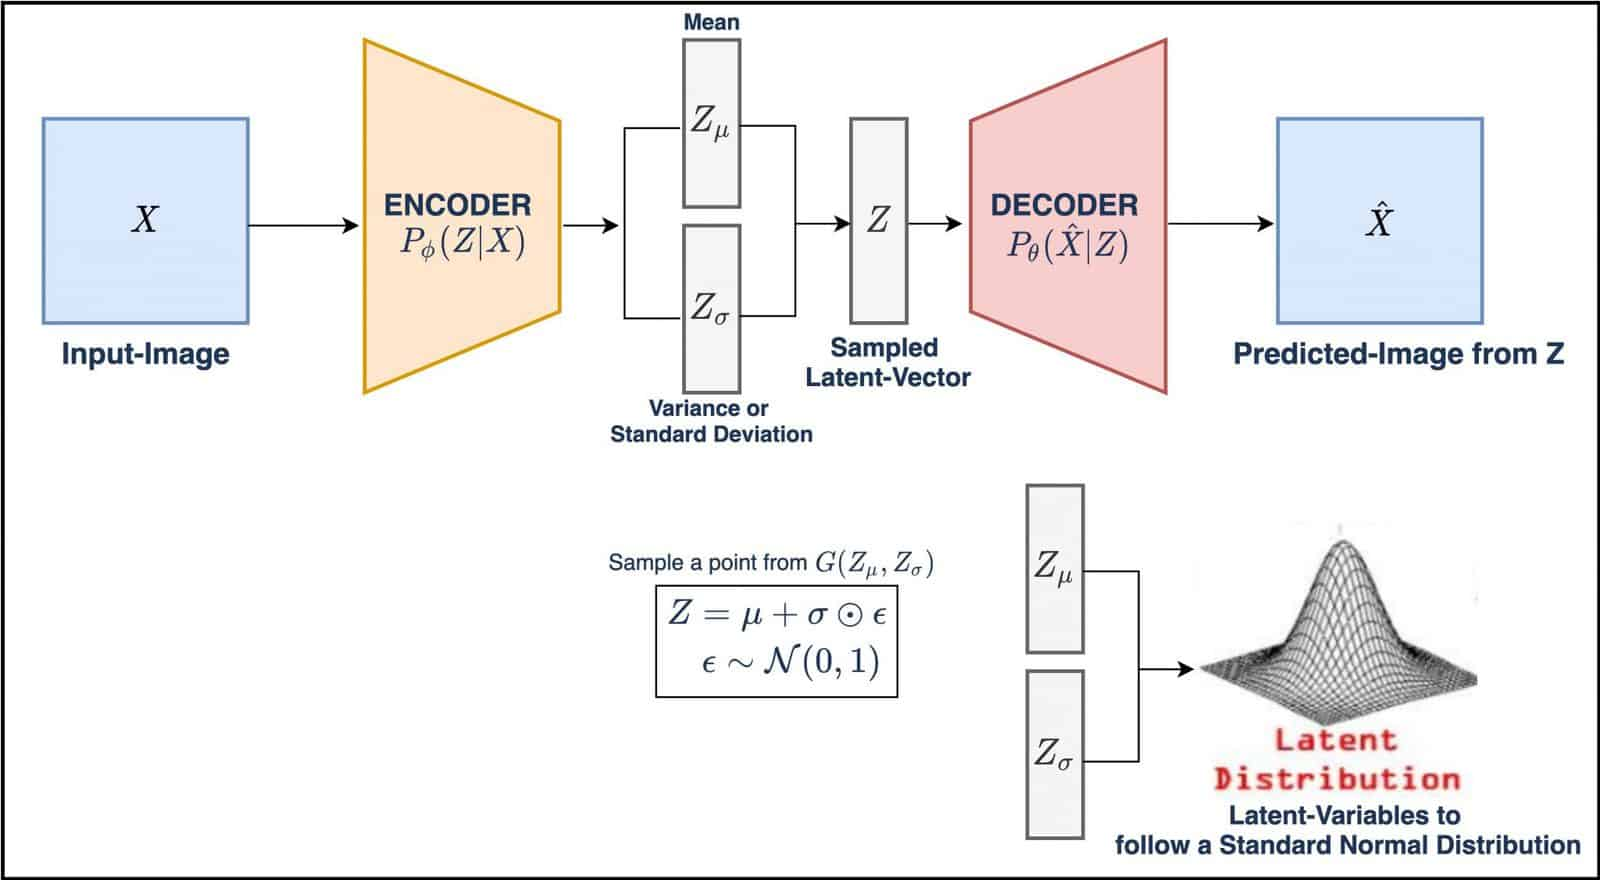
\includegraphics[width=0.8\textwidth]{arch.jpg}
\end{figure}

A Variational Autoencoder consists of:
\begin{itemize}
    \item An encoder network $q_{\phi}(z|x)$ that maps input $x$ to a latent distribution.
    \item A decoder network $p_{\theta}(x|z)$ that reconstructs data from latent variable $z$.
\end{itemize}

Latent variables $z$ are sampled from a prior $p(z)$, typically a standard normal distribution:
\[
p(z) = \mathcal{N}(0, I)
\]

The encoder produces parameters $\mu(x)$ and $\sigma^2(x)$ to approximate a Gaussian posterior distribution over latent variable $z$ given input $x$:
\[
q_{\phi}(z|x) = \mathcal{N}(z; \mu_{\phi}(x), \mathrm{diag}(\sigma^2_{\phi}(x)))
\]

where $\mu(x)$ is the mean and $\sigma^2(x)$ is the variance of the latent variable, $\phi$ are the parameters of the encoder network, and the covariance matrix is diagonal.

\section*{Objective Function}

The variational lower bound (ELBO) on the log-likelihood $\log p_{\theta}(x)$ is:
\[
\log p_{\theta}(x) \geq \mathbb{E}_{q_{\phi}(z|x)}[\log p_{\theta}(x|z)] - \mathrm{KL}(q_{\phi}(z|x) \| p(z))
\]

\begin{itemize}
    \item Reconstruction loss: $\mathbb{E}_{q_{\phi}(z|x)}[\log p_{\theta}(x|z)]$
    \item Regularization: $\mathrm{KL}(q_{\phi}(z|x) \| p(z))$
\end{itemize}

\section*{KL Divergence Term}

For Gaussian posterior and standard normal prior:
\[
\mathrm{KL}(q_{\phi}(z|x) \| p(z)) = \frac{1}{2} \sum_{i=1}^{d} \left( \mu_i^2 + \sigma_i^2 - \log \sigma_i^2 - 1 \right)
\]

\section*{Reparameterization Trick}

To backpropagate through the sampling process:
\[
z = \mu + \sigma \odot \epsilon, \quad \epsilon \sim \mathcal{N}(0, I)
\]

This allows rewriting the expectation:
\[
\mathbb{E}_{q_{\phi}(z|x)}[\log p_{\theta}(x|z)] \approx \frac{1}{L} \sum_{l=1}^{L} \log p_{\theta}(x | z^{(l)})
\]
with $z^{(l)} = \mu + \sigma \odot \epsilon^{(l)}$

\section*{Final Loss Function}

The total loss to minimize (negative ELBO):
\[
\mathcal{L}_{\text{VAE}}(x) = -\mathbb{E}_{q_{\phi}(z|x)}[\log p_{\theta}(x|z)] + \mathrm{KL}(q_{\phi}(z|x) \| p(z))
\]

\end{document}
